\section{Messergebnisse und Auswertung}
\subsection{Allgemeines}
\subsubsection{Fehler und Zählrate}
\label{subsub:errorsandcounts}
Die Anzahl $N$ der Messereignisse von einem Kanal des MCAs ist poissonverteilt. Daher gilt für den Fehler $s_N$:
\begin{equation}
\label{eq:poisson:error}
  s_N = \sqrt{N}
\end{equation} 
Die Fehler wurden nur in den Graphiken für die Fits gezeichnet, damit beurteilt werden kann, ob der durchgeführte Fit die Messwerte innerhalb
ihrer Fehler beschreibt. Bei den Übersichten von den Gesamtspektren sind die Fehler weggelassen worden, um einen besseren Überblick zu gewähren. \\[\baselineskip]
Aufgrund der unterschiedlichen Messzeiten wird die Anzahl $N$ der Messereignisse durch die verstrichene Zeit $t$\footnote{ohne Totzeit}
auf eine Zählrate $n$ normiert. Dementsprechend werden auch die Fehler $s_N$ angepasst.
\begin{equation}
\label{eq:countrate}
  n = \frac{N}{t}, \qquad s_n = \frac{s_N}{t}
\end{equation}

\subsubsection{Gauß-Verteilung}
\label{subsub:gaus}
Bei der Auswertung wird oft die Gauß-Verteilung als theoretisches Modell (also auch als Fit-Modell) der Messwerte verwendet. Es wird folgende 
Konvention eingeführt:
\begin{equation}
  \label{eq:gaus}
  \gaus(x; A, c, s) = A \cdot e^{-\frac{1}{2} \left( \frac{x - c}{s} \right)^2}
\end{equation}
wobei $\gaus(x; A, c, s)$ eine Funktion von $x$ mit Parametern $A$ (Amplitude), $c$ (Erwartungswert\footnote{$c=$ channel}) und 
$s$ (Standardabweichung) ist.

\subsection{\textgamma-Spektrum des Untergrunds}
Das Untergrundspektrum ist in \autoref{img:underground:spectrum} abgebildet. Man erkennt einen Peak bei Kanal 3600, der aufgrund der noch 
fehlenden Energieeichung erst in \ref{sub:eval:undergroundpeak} diskutiert wird. Bei kleineren Kanälen (was einer kleineren Energie entspricht) ist 
die Zählrate tendenziell höher, was auf eine höhere Anzahl von niederenergetischer Strahlung zurückzuführen ist. 
\begin{figure}[H]
\begin{center}
  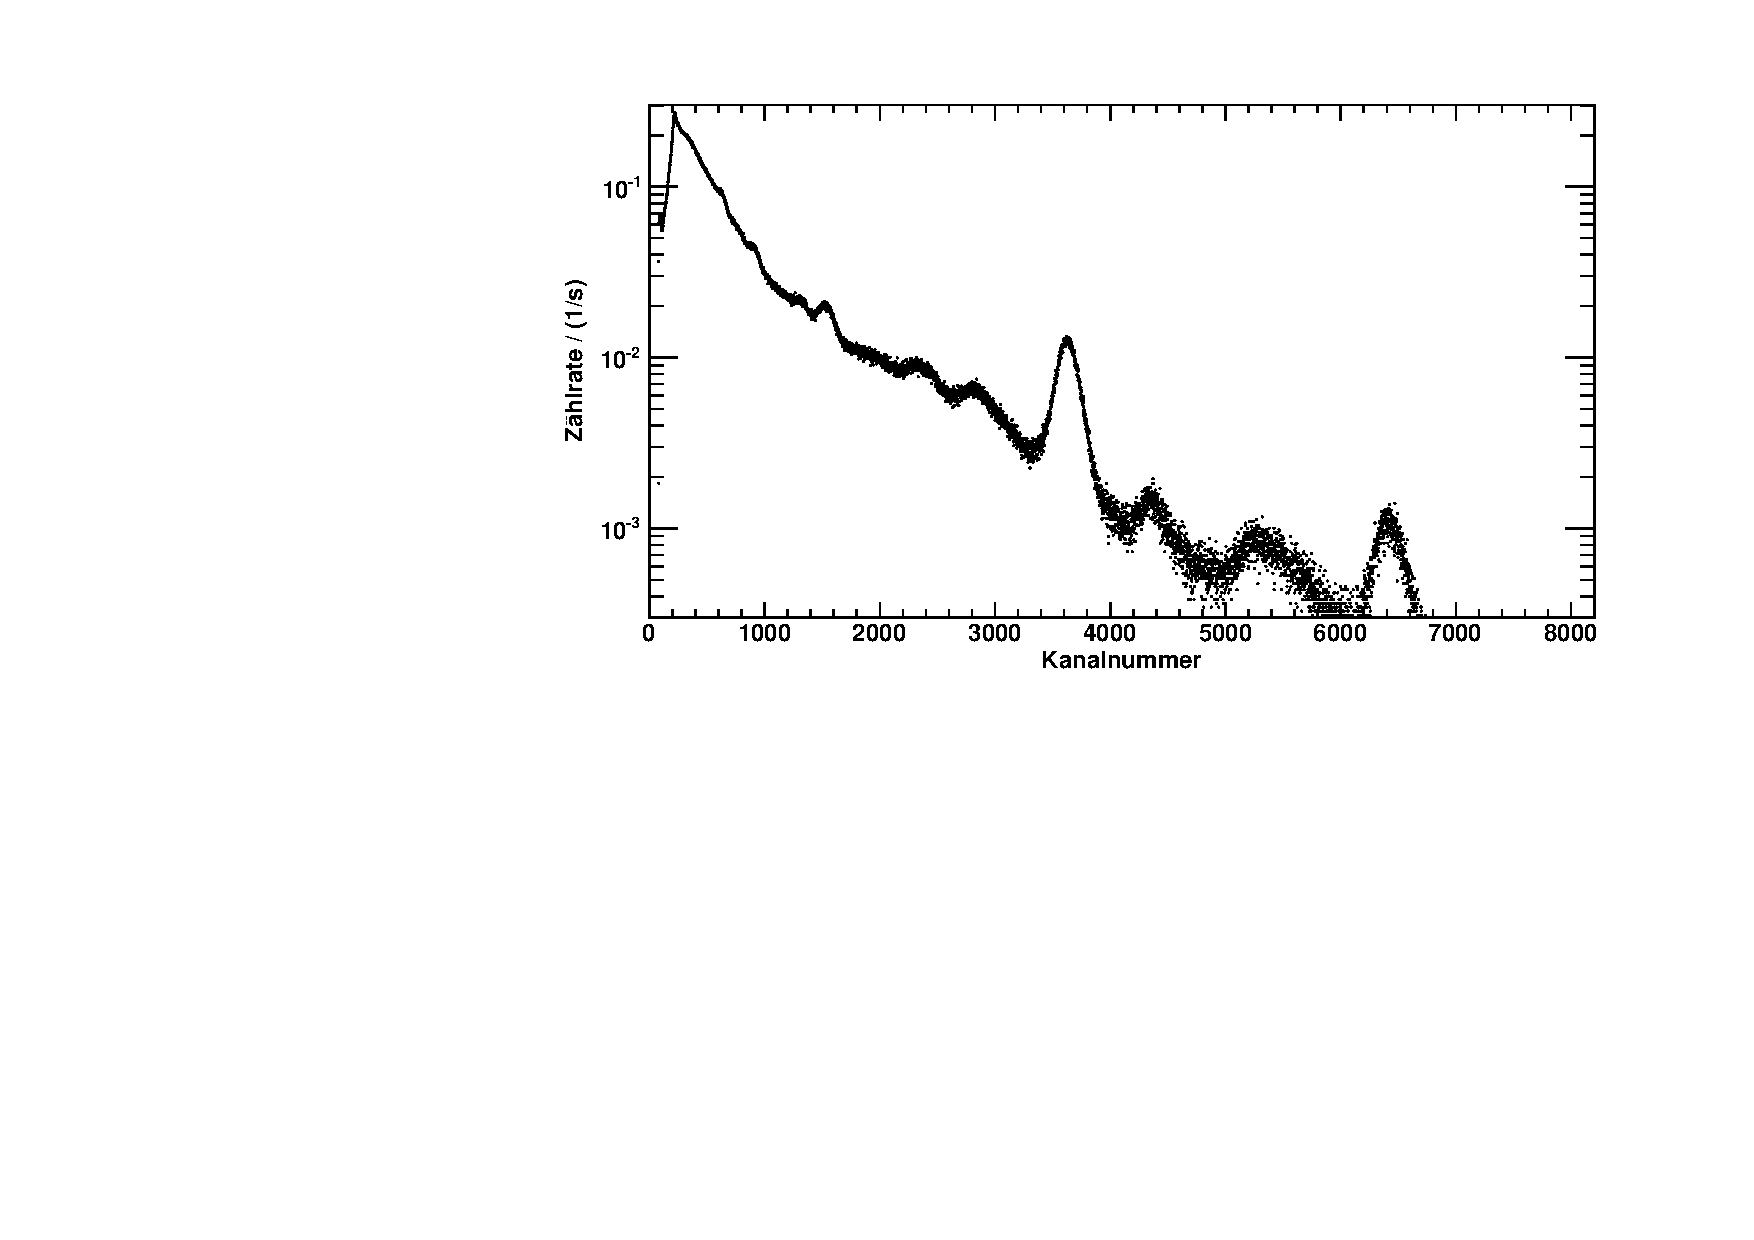
\includegraphics[width=\textwidth]{../img/underground_spectrum.pdf}
  \caption{Untergrund}
  \label{img:underground:spectrum}
\end{center}
\end{figure}
Um eine gute Auswertung der Messungen zu erreichen, ist es notwendig den Untergrund $u$ von den gemessenen Werten $n'$ abzuziehen. Man erhält 
somit untergrundbereinigte Messwerte $n$. Der Fehler auf diese wird mit der Gauß'schen Fehlerfortpflanzung berechnet.
\begin{equation}
  n = n' - u, \qquad s_n = \sqrt{s_{n'}^2 + s_u^2}
\end{equation}
Im folgenden sind alle Spektren untergrundbereinigt.

\subsection{Energieeichung des MCAs}
\subsubsection{\na-Peaks}
Das gesamte Spektrum von \na\,ist in \autoref{img:na:spectrum} dargestellt. Da sich die Probe von \na\, von den anderen unterscheidet, konnten nicht die 
gleichen Bedingungen wie bei der Untergrundmessung hergestellt werden. Der als Halterung und zur Abschirmung verwendete Bleiblock konnte nicht 
benutzt werden. Deshalb ist trotz Bereinigung des Untergrundes noch ein Untergrund zu sehen. Vor allem die ansonsten vom Bleiblock abgeschirmte 
niederenergetische Strahlung sticht dabei besonders hervor. Außerdem gibt es aus dem gleichen Grund auch einige negative Zählraten, welche jedoch 
außerhalb von den für uns relevanten Bereichen liegen.
\begin{figure}[H]
\begin{center}
  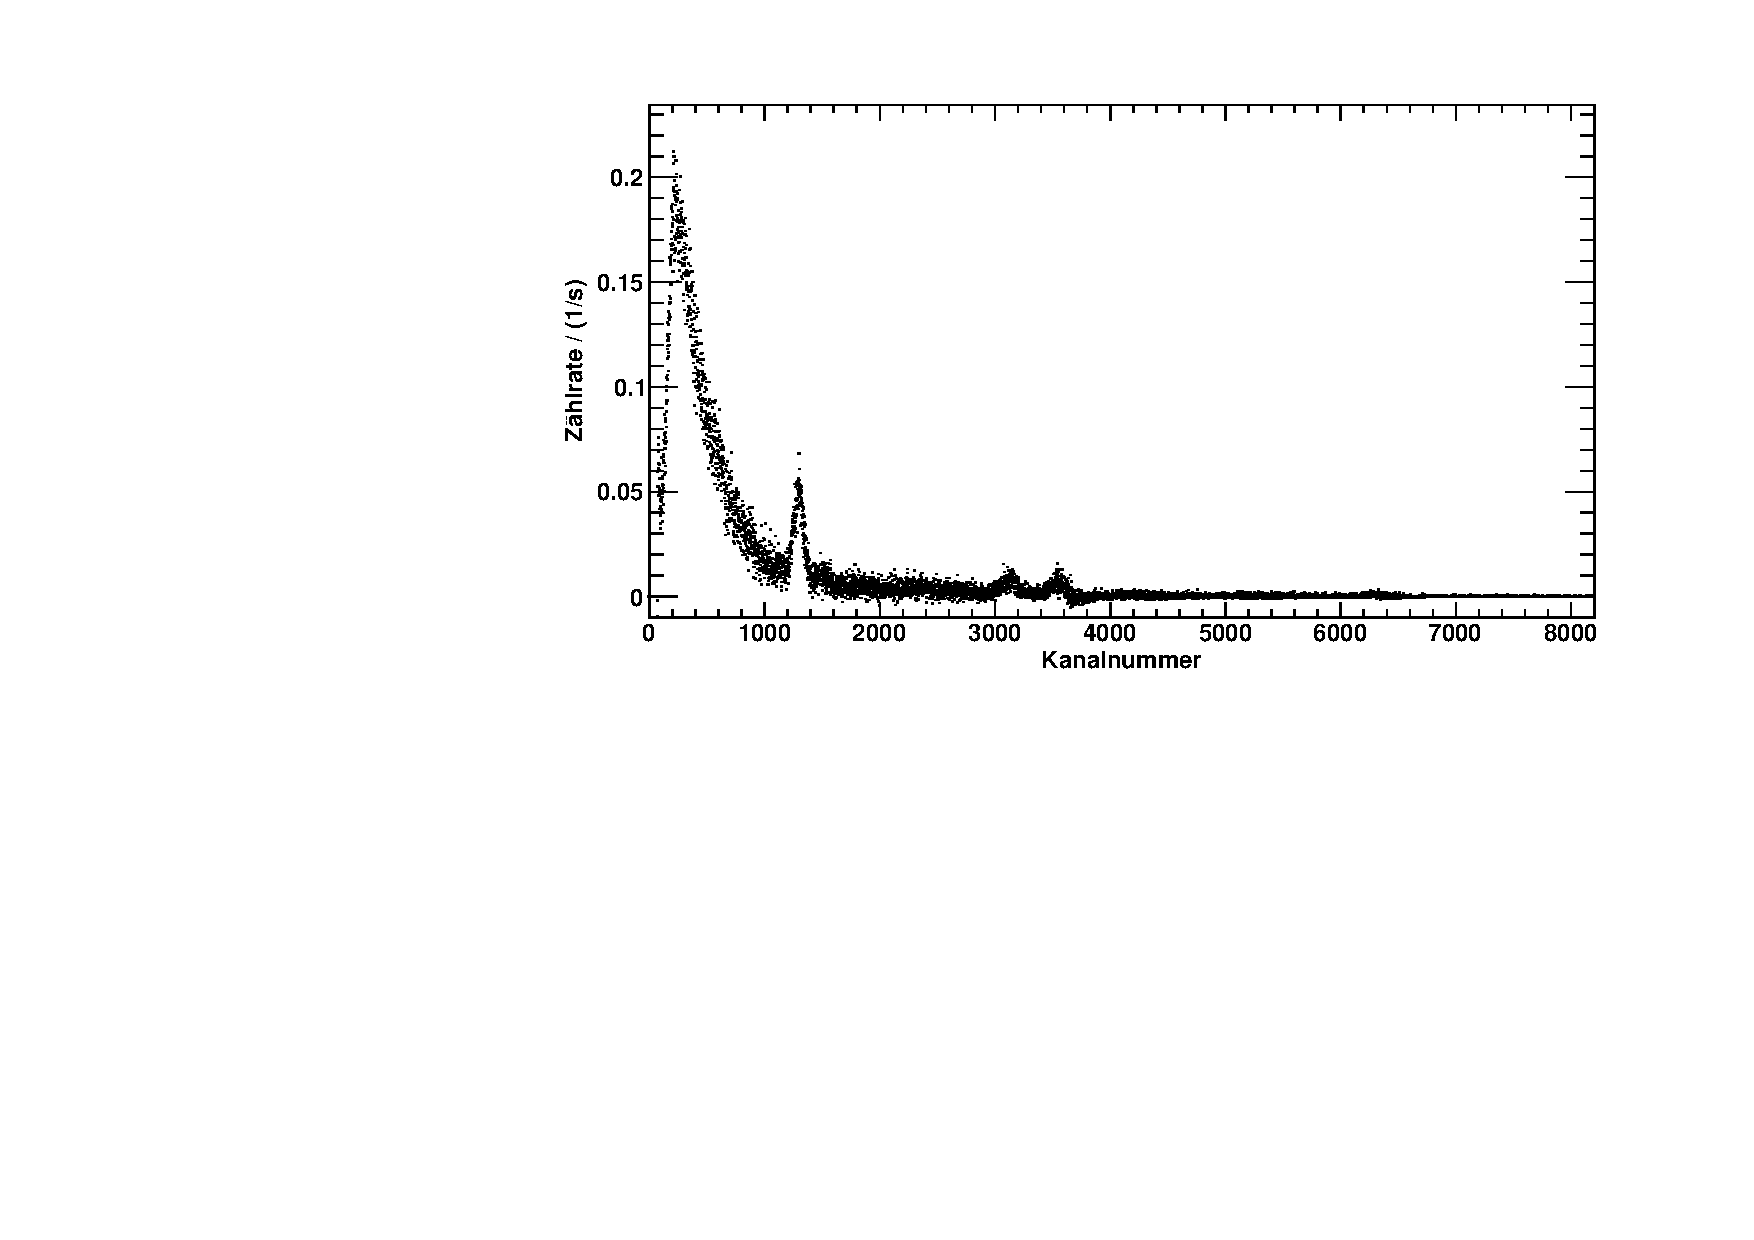
\includegraphics[width=\textwidth]{../img/na_spectrum.pdf}
  \caption{\textgamma-Spektrum von \chemel{Na}{22}}
  \label{img:na:spectrum}
\end{center}
\end{figure}
Trotz des nichtverschwindenden Untergrundes lässt sich der 511\,keV-PEak gut erkennen. Des weiteren sind zwei weitere Peaks mit geringerer 
Zählrate bei Kanal 3100 und 3500 zu erkennen. Ein Vergleich mit dem Spektrum des Untergrundes \autoref{img:underground:spectrum} identifiziert 
den zweiten Peak als Folge des Untergrundes (und nicht vollständiger Abschirmung dessen). Damit kann der erste Peak \na\,zugeordnet werden.\\[\baselineskip]
Die beiden Peaks von \na\, werden nun jeweils mit einer Gauß-Verteilung \\(\autoref{eq:gaus}), verziert mit einem linearen Untergrund, 
gefittet, um den genauen Kanal des Maximums zu bestimmen.
\begin{equation}
  y = a + b\cdot x + \gaus()
\end{equation}
\begin{figure}[H]
\begin{center}
  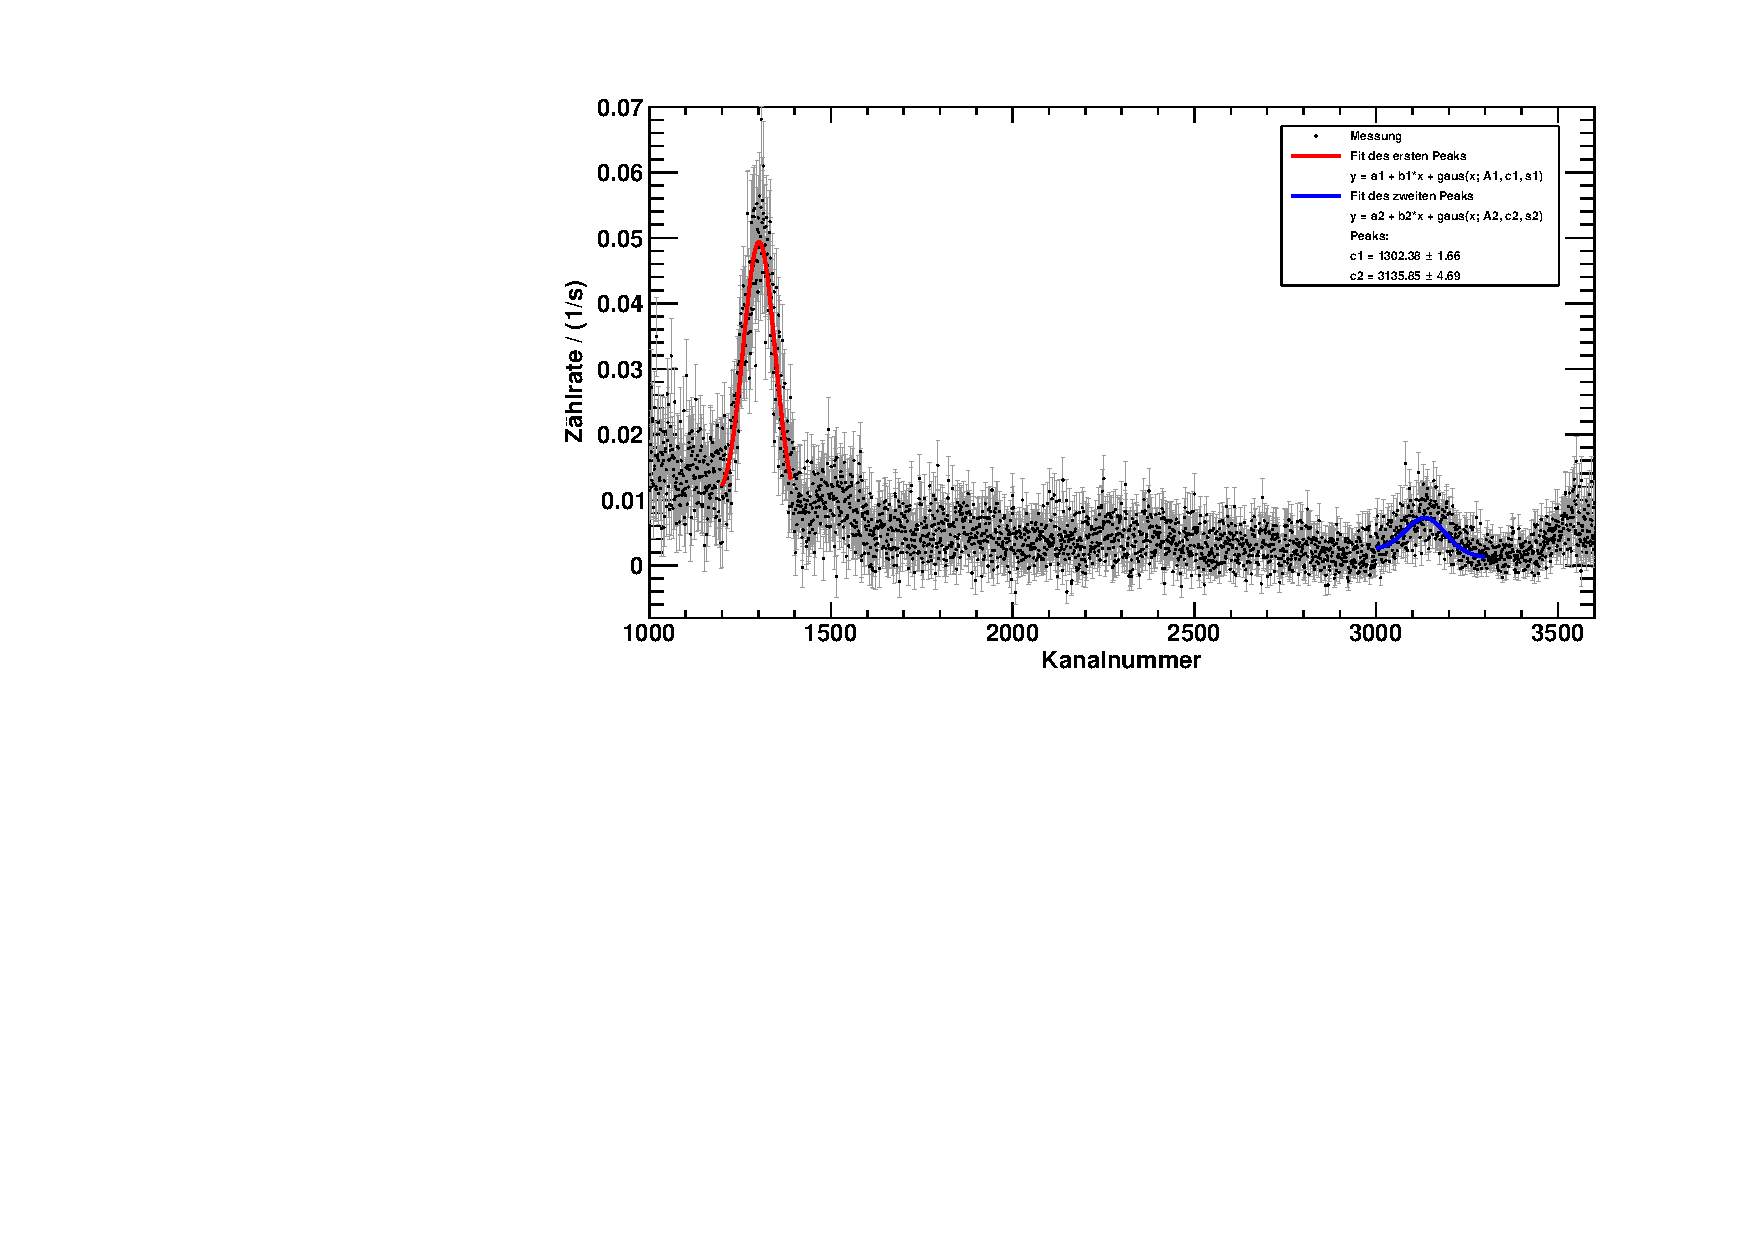
\includegraphics[width=\textwidth]{../img/na_peaks.pdf}
  \caption{\textgamma-Spektrum von \chemel{Na}{22} mit 511\,keV- und 1274\,keV-Peak}
  \label{img:na:peaks}
\end{center}
\end{figure}

\subsubsection{\co-Peaks}
\begin{figure}[H]
\begin{center}
  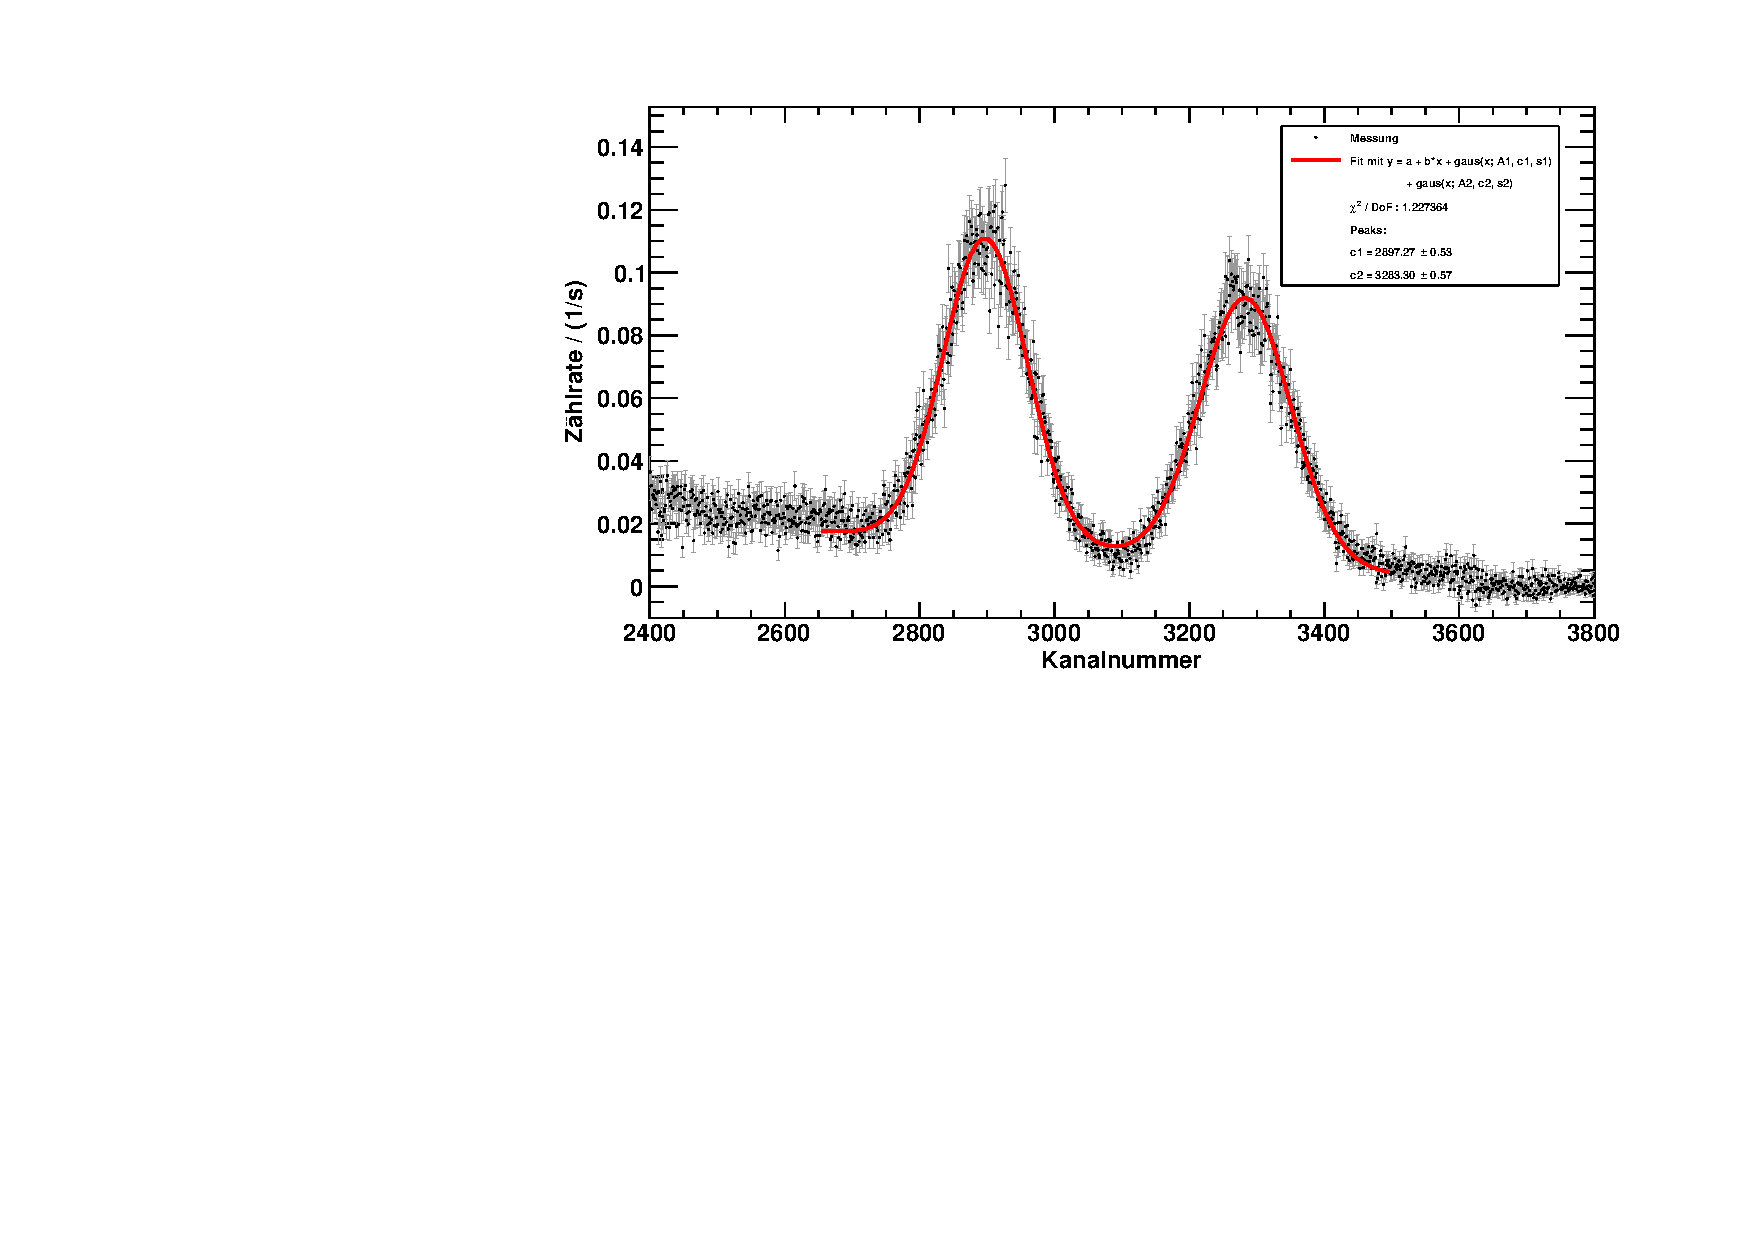
\includegraphics[width=\textwidth]{../img/co_peaks.pdf}
  \caption{\textgamma-Spektrum von \chemel{Co}{60}}
  \label{img:co:peak}
\end{center}
\end{figure}

\subsubsection{\eu-Peaks}
\begin{figure}[H]
\begin{center}
  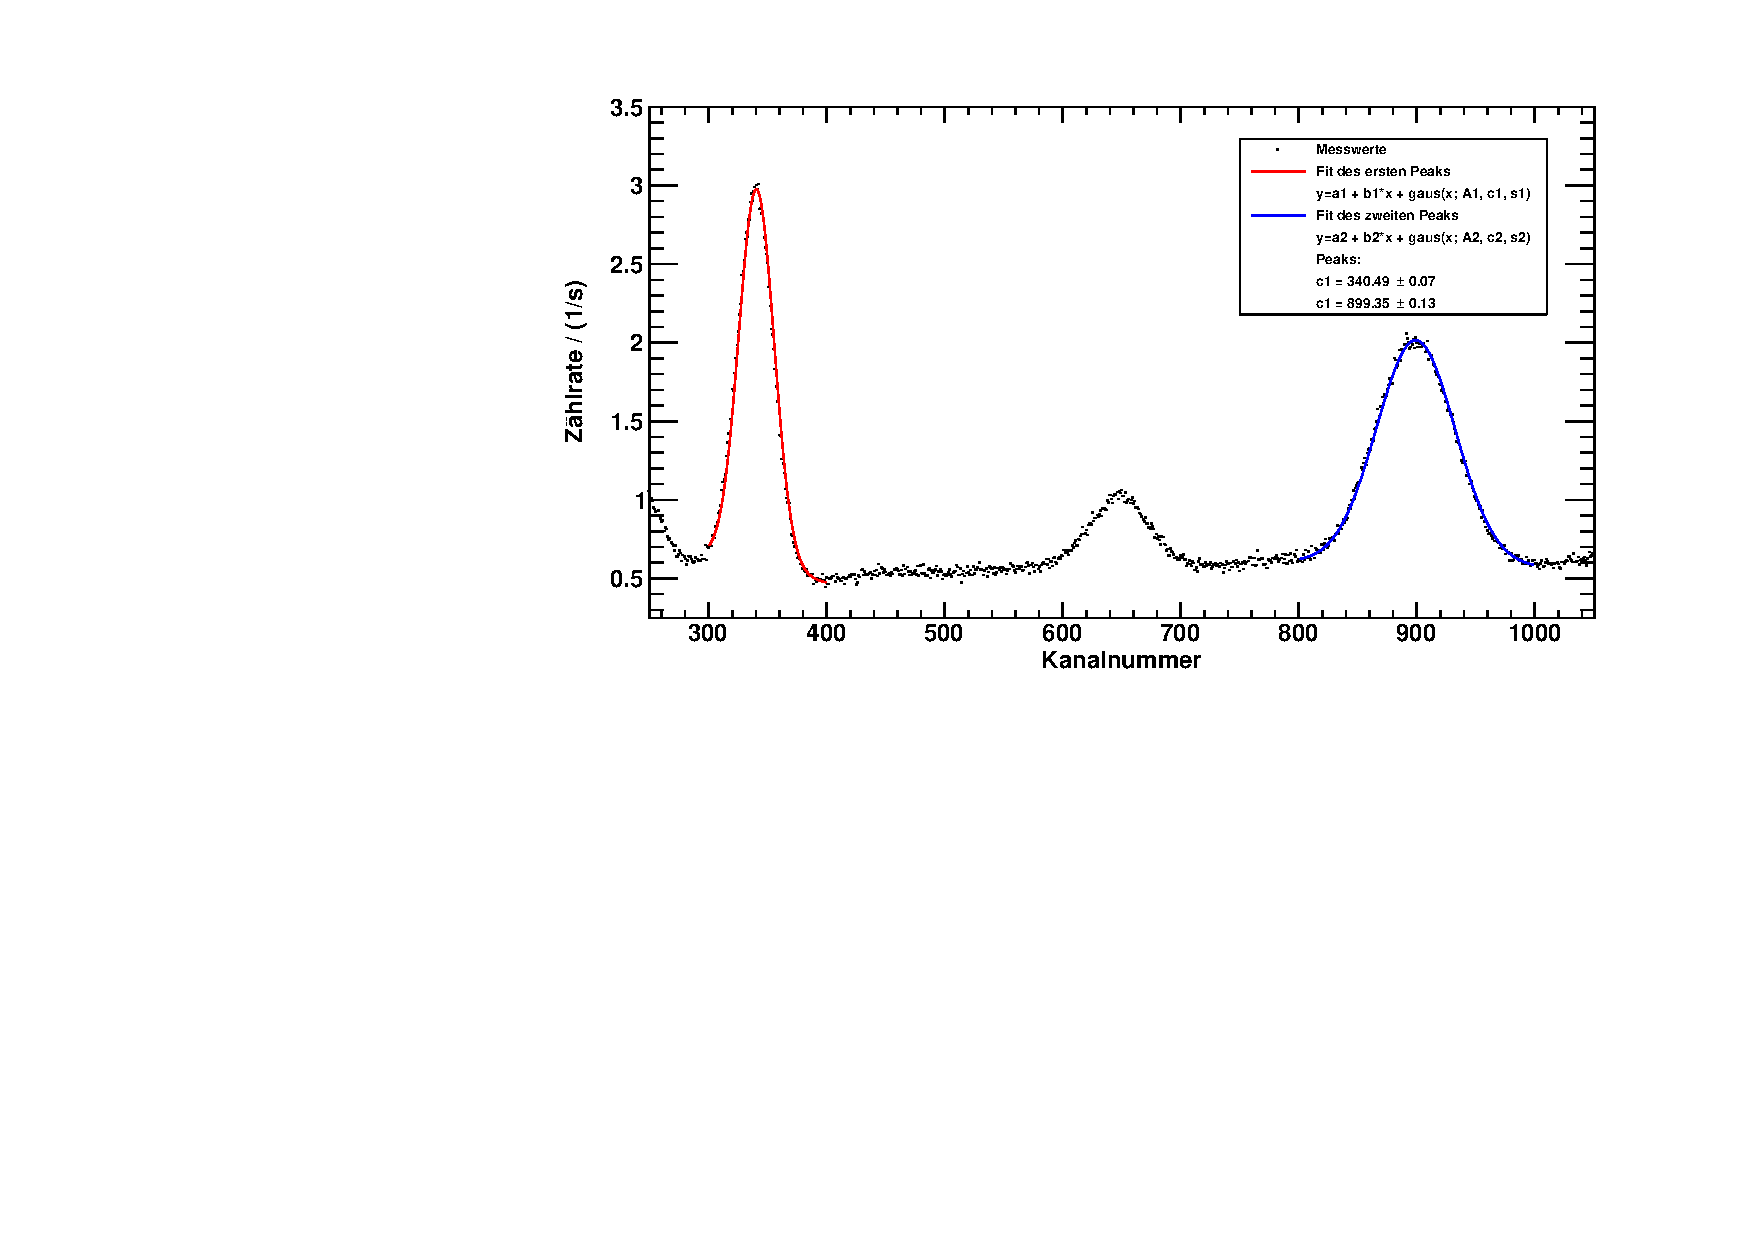
\includegraphics[width=\textwidth]{../img/eu_peaks.pdf}
  \caption{\textgamma-spektrum von \chemel{Eu}{152}}
  \label{img:eu:peak}
\end{center}
\end{figure}

\begin{figure}[H]
\begin{center}
  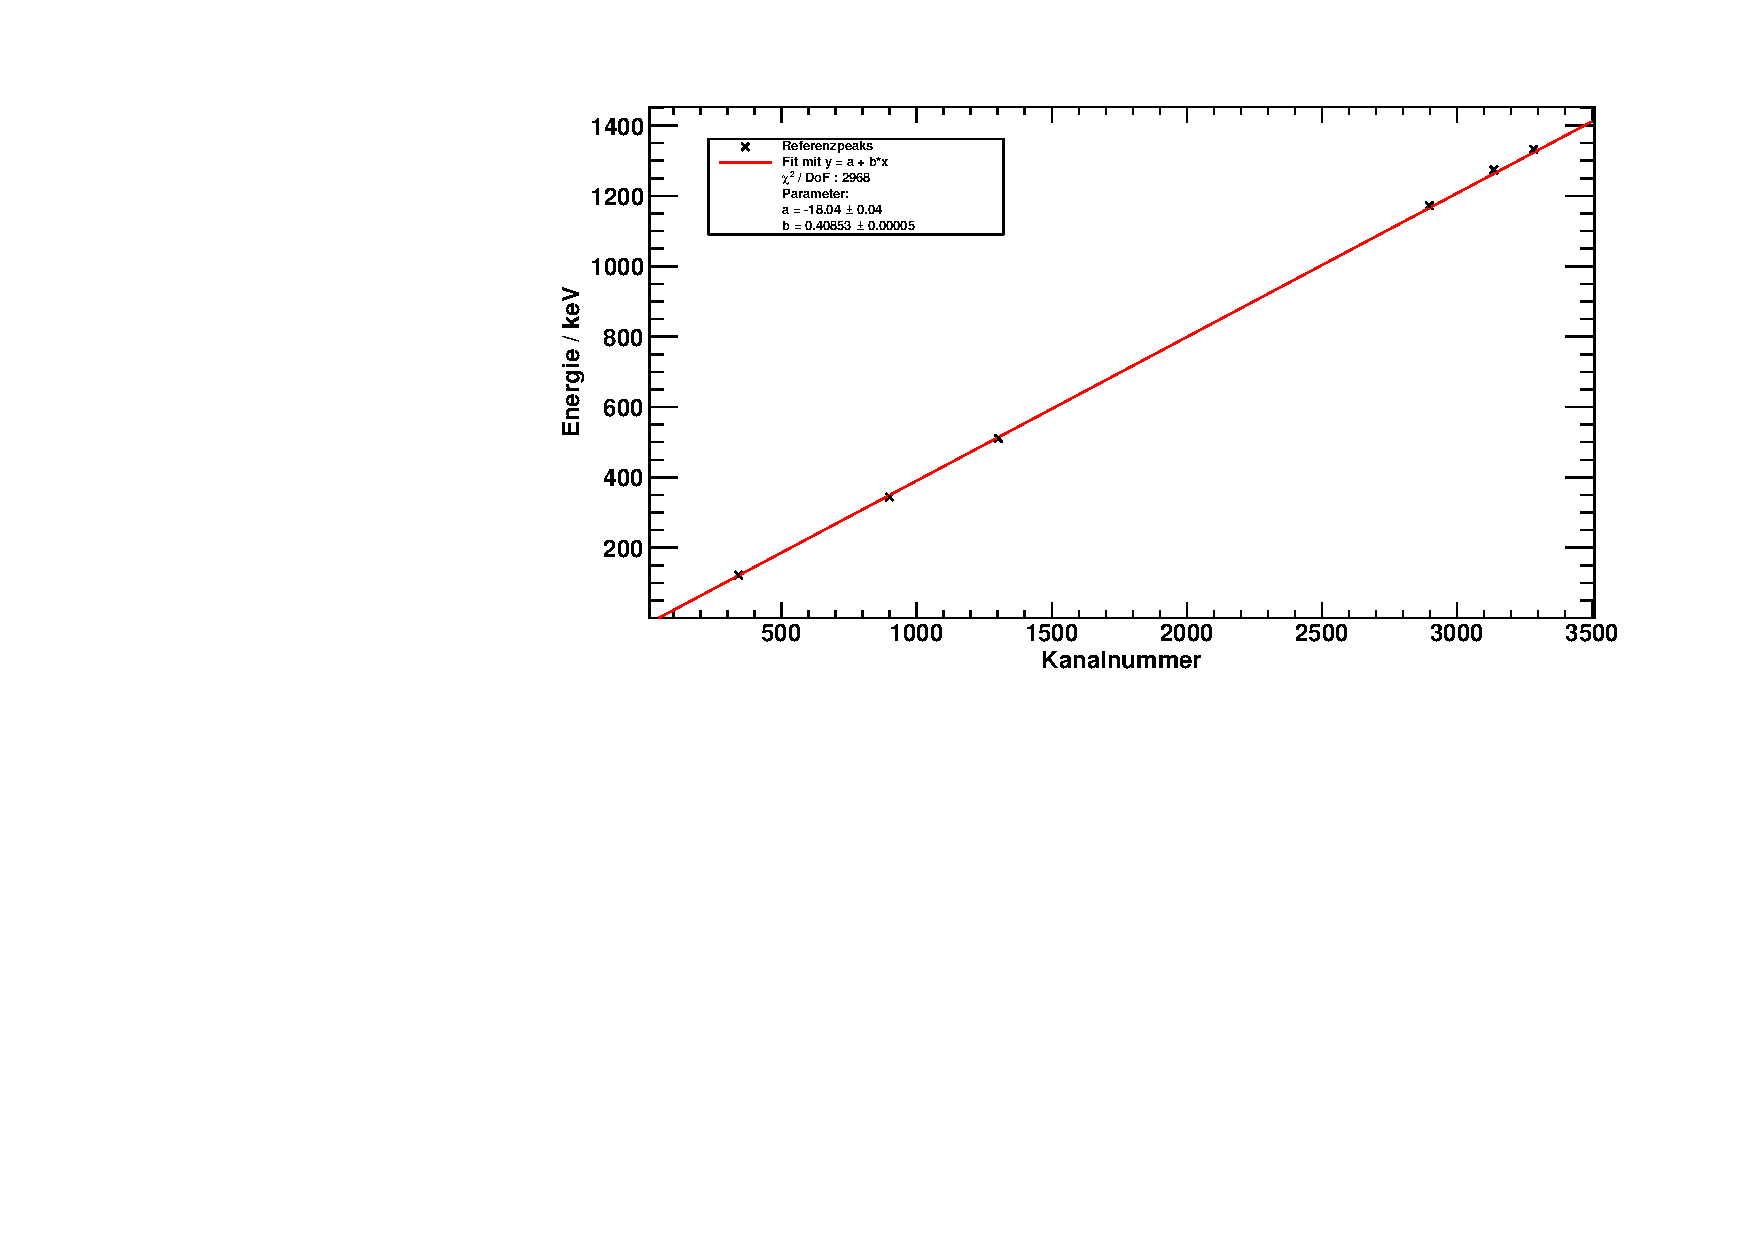
\includegraphics[width=\textwidth]{../img/energy_gauge_lin.pdf}
  \caption{Lineare Energieeichung}
  \label{img:gauge:lin}
\end{center}
\end{figure}

\begin{figure}[H]
\begin{center}
  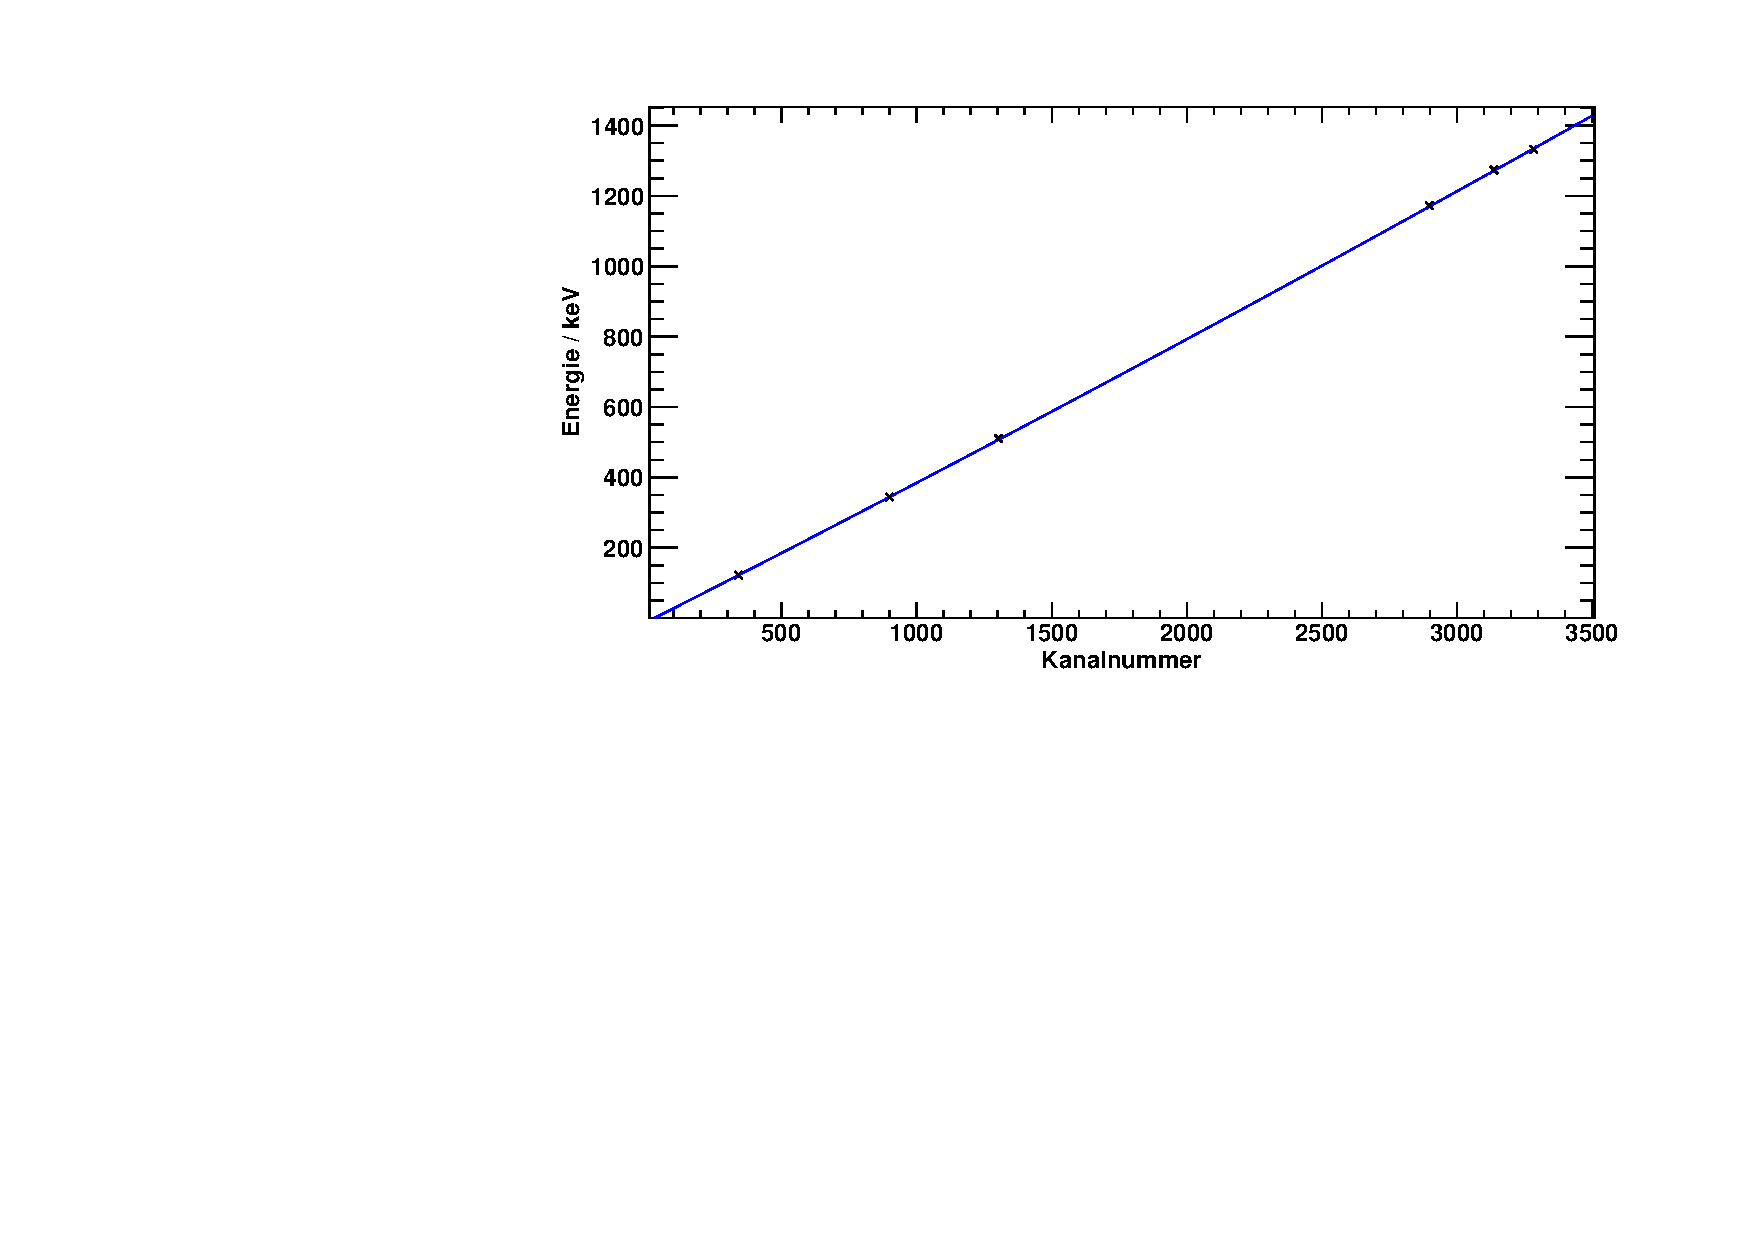
\includegraphics[width=\textwidth]{../img/energy_gauge_quad.pdf}
  \caption{Quadratische Energieeichung}
  \label{img:gauge:quad}
\end{center}
\end{figure}

\subsection{\textgamma-Spektrum von \chemel{Th}{228}}
\begin{figure}[H]
\begin{center}
  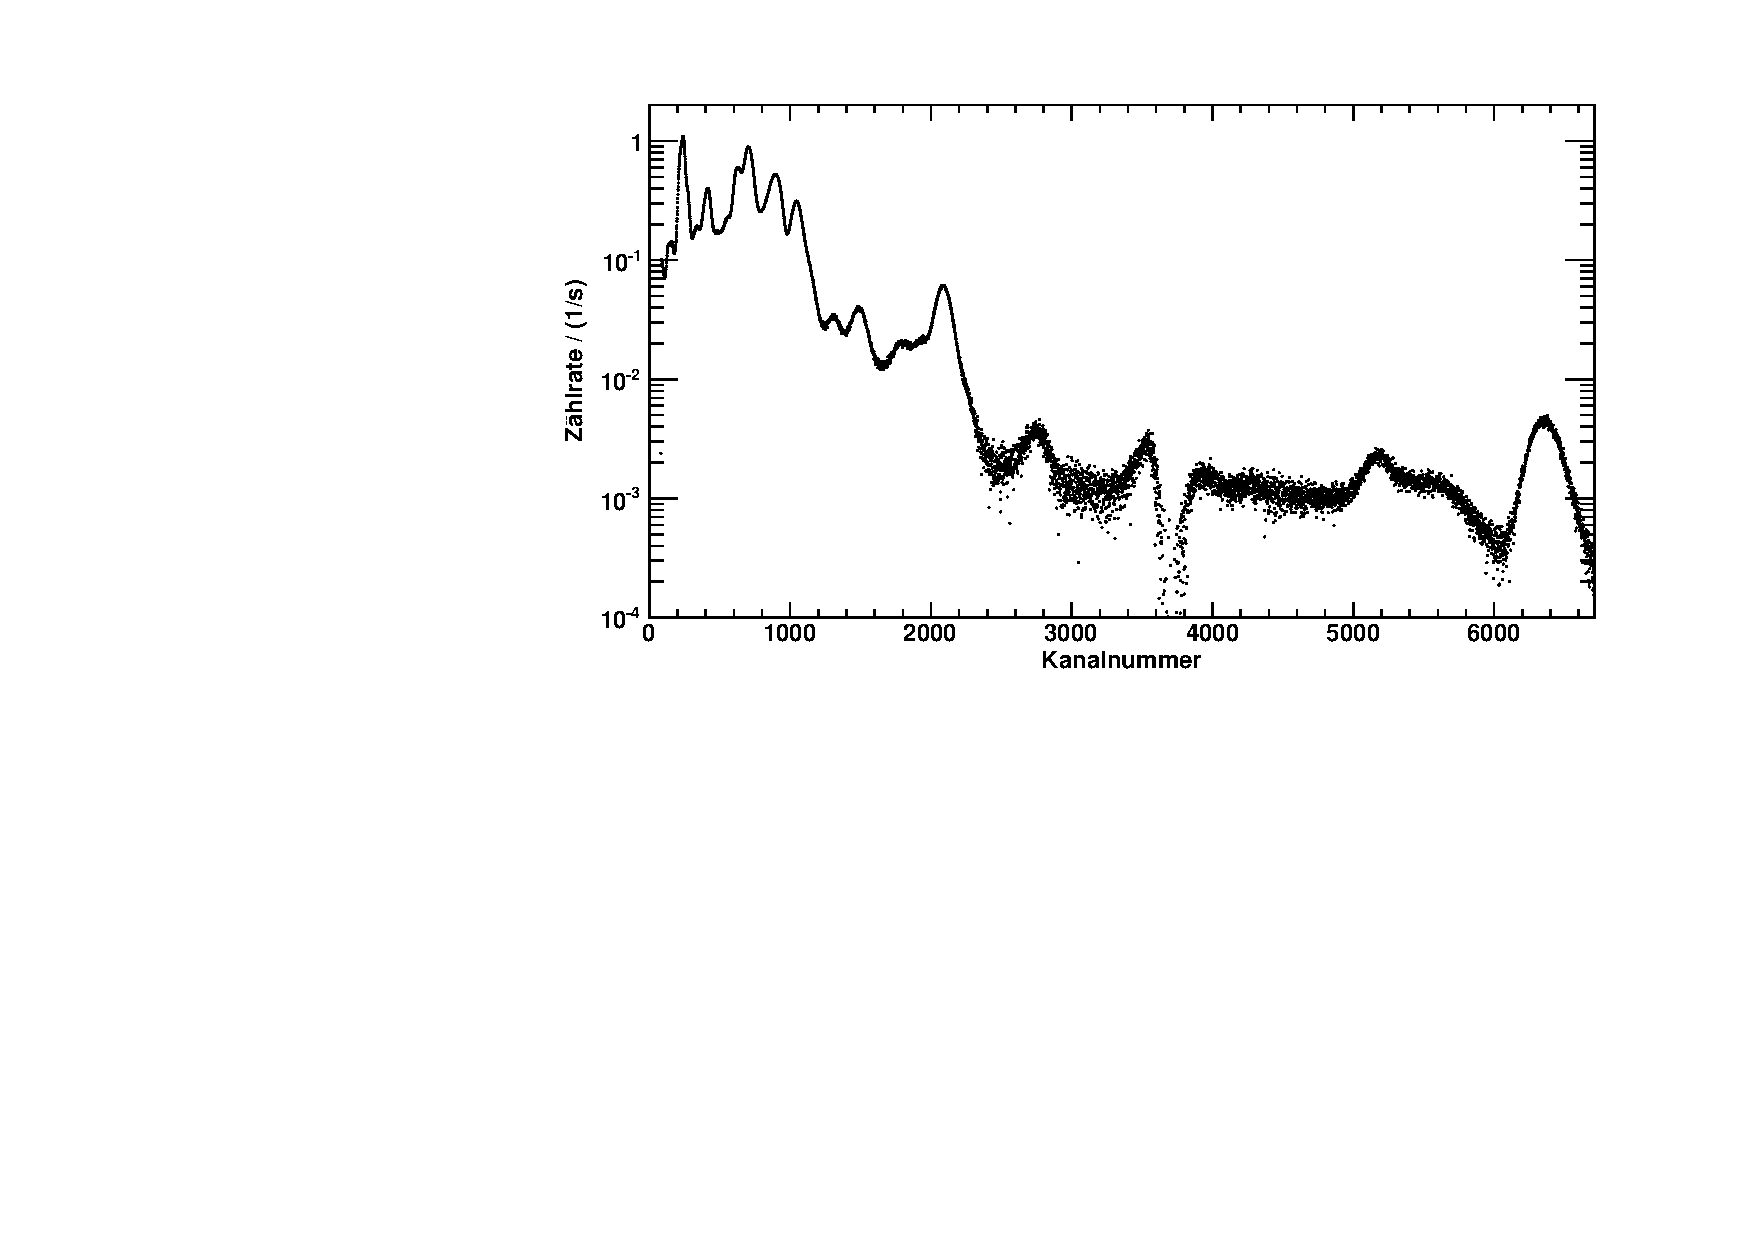
\includegraphics[width=\textwidth]{../img/th_energyspectrum.pdf}
  \caption{\textgamma-Spektrum von \chemel{Th}{228}}
  \label{img:th:spectrum}
\end{center}
\end{figure}

\subsubsection{Single-Peak Fit} % TODO Benennung
\begin{figure}[H]
\begin{center}
  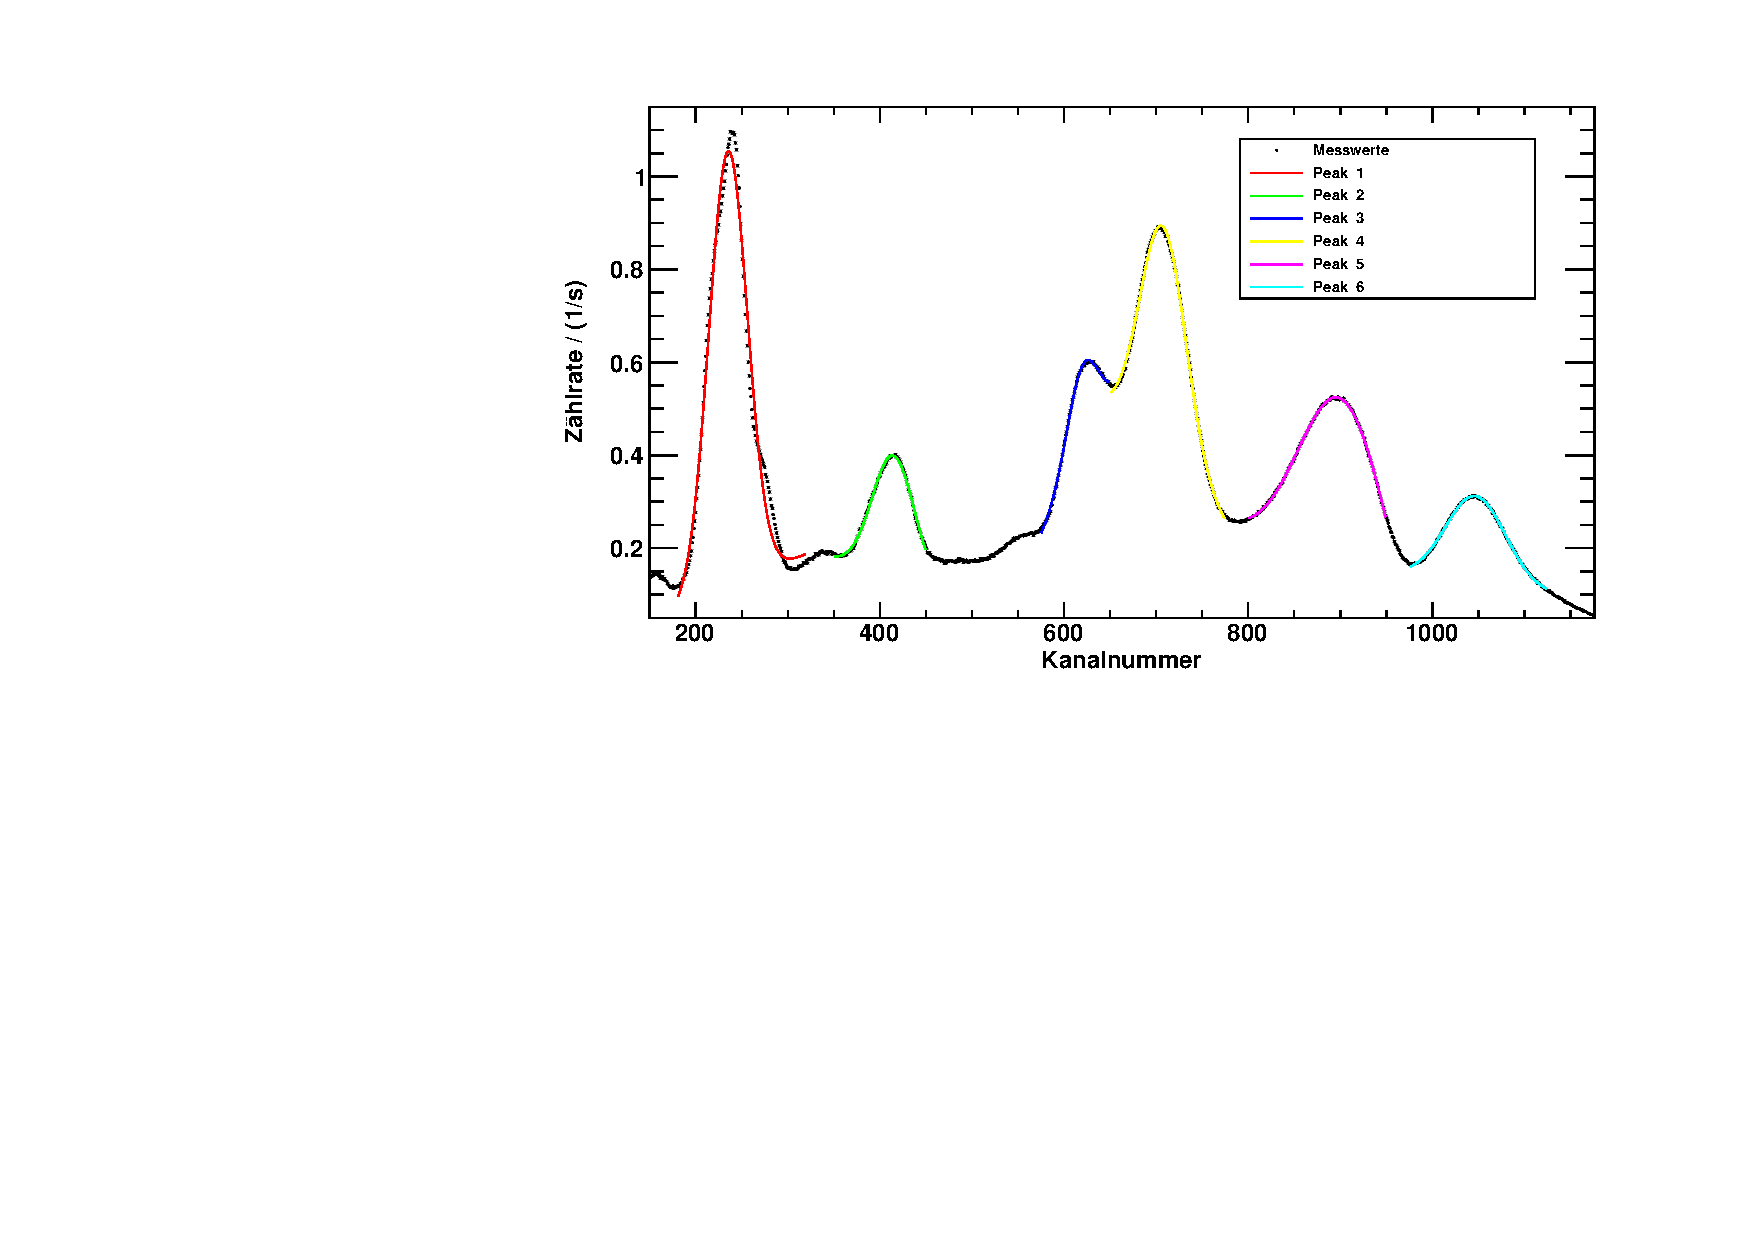
\includegraphics[width=\textwidth]{../img/th_peaks_single_01-06.pdf}
  \caption{Peaks 1 bis 6}
  \label{img:th:peaks:single:0106}
\end{center}
\end{figure}

\begin{figure}[H]
\begin{center}
  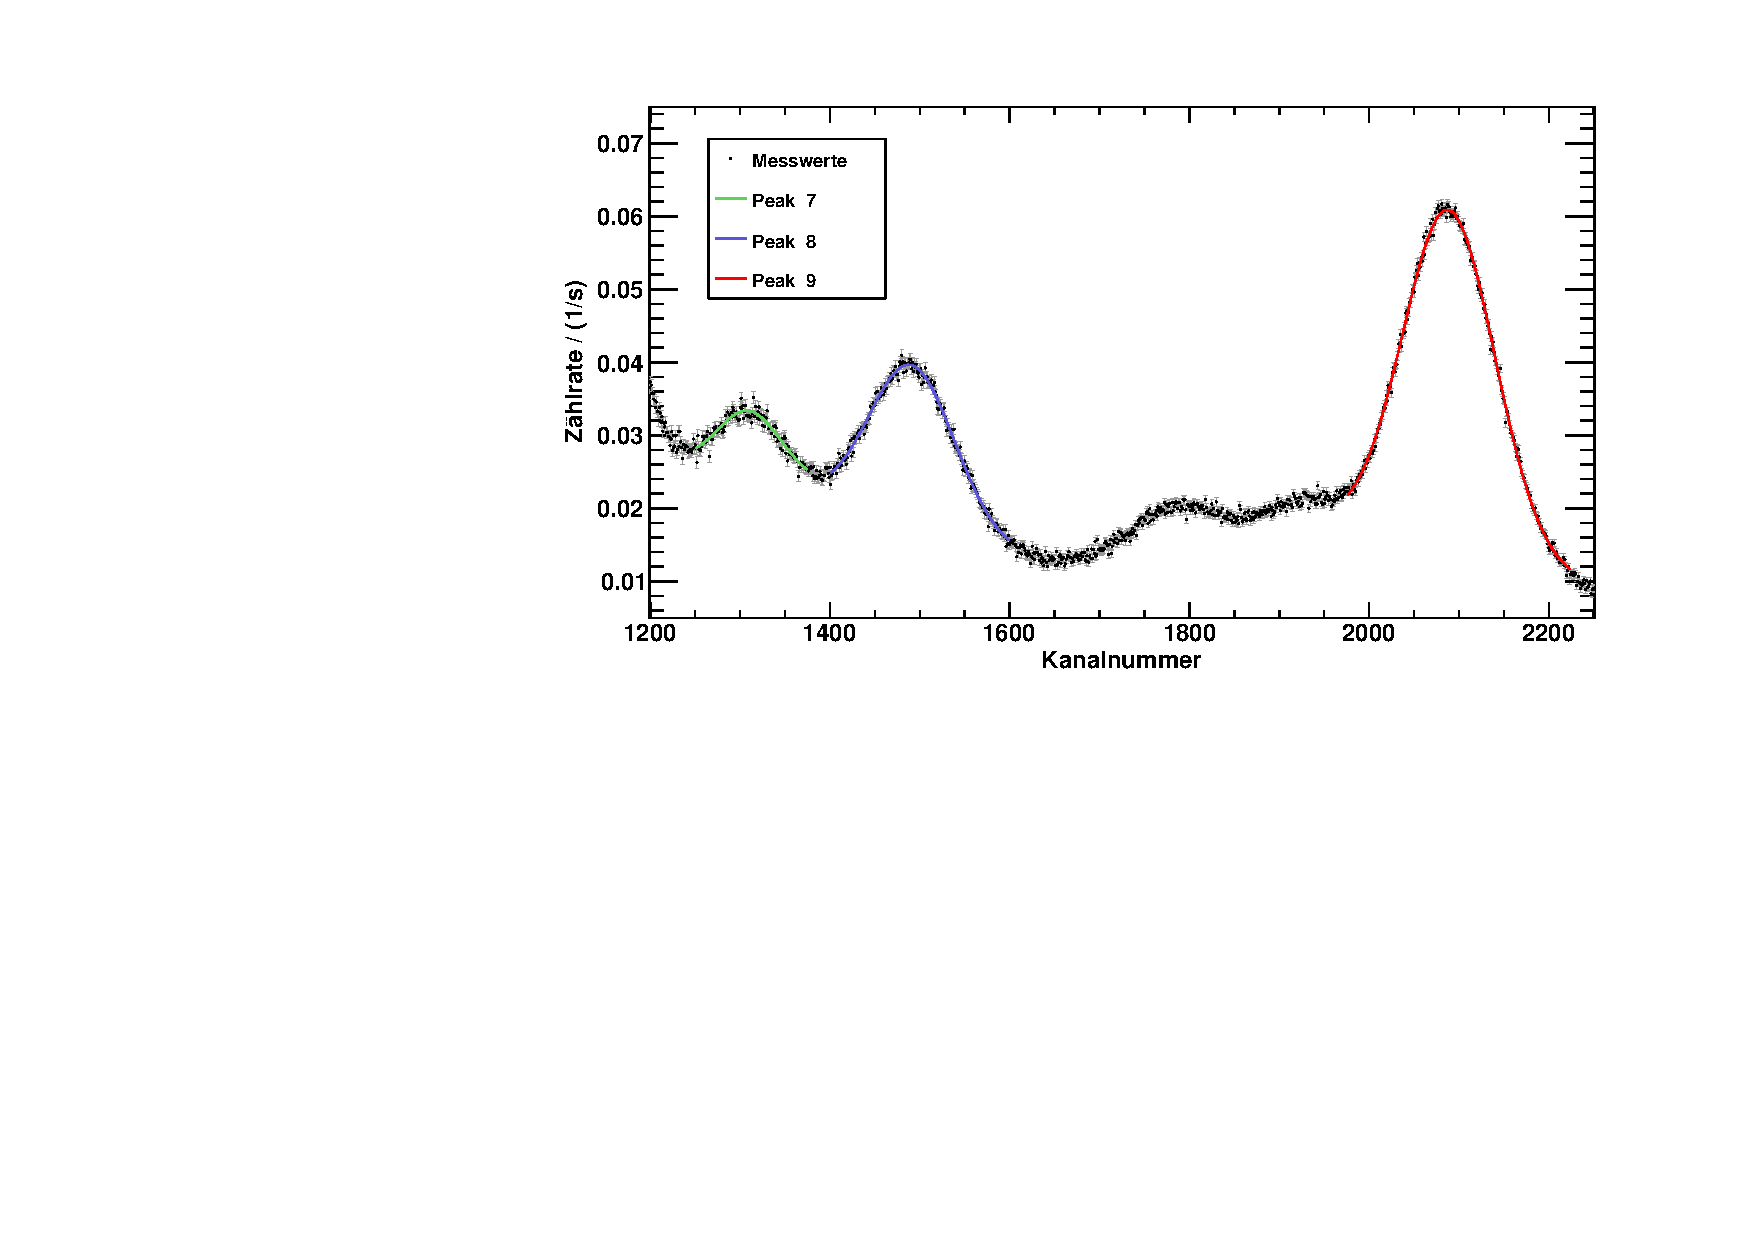
\includegraphics[width=\textwidth]{../img/th_peaks_single_07-09.pdf}
  \caption{Peaks 7 bis 9}
  \label{img:th:peaks:single:0709}
\end{center}
\end{figure}

\begin{figure}[H]
\begin{center}
  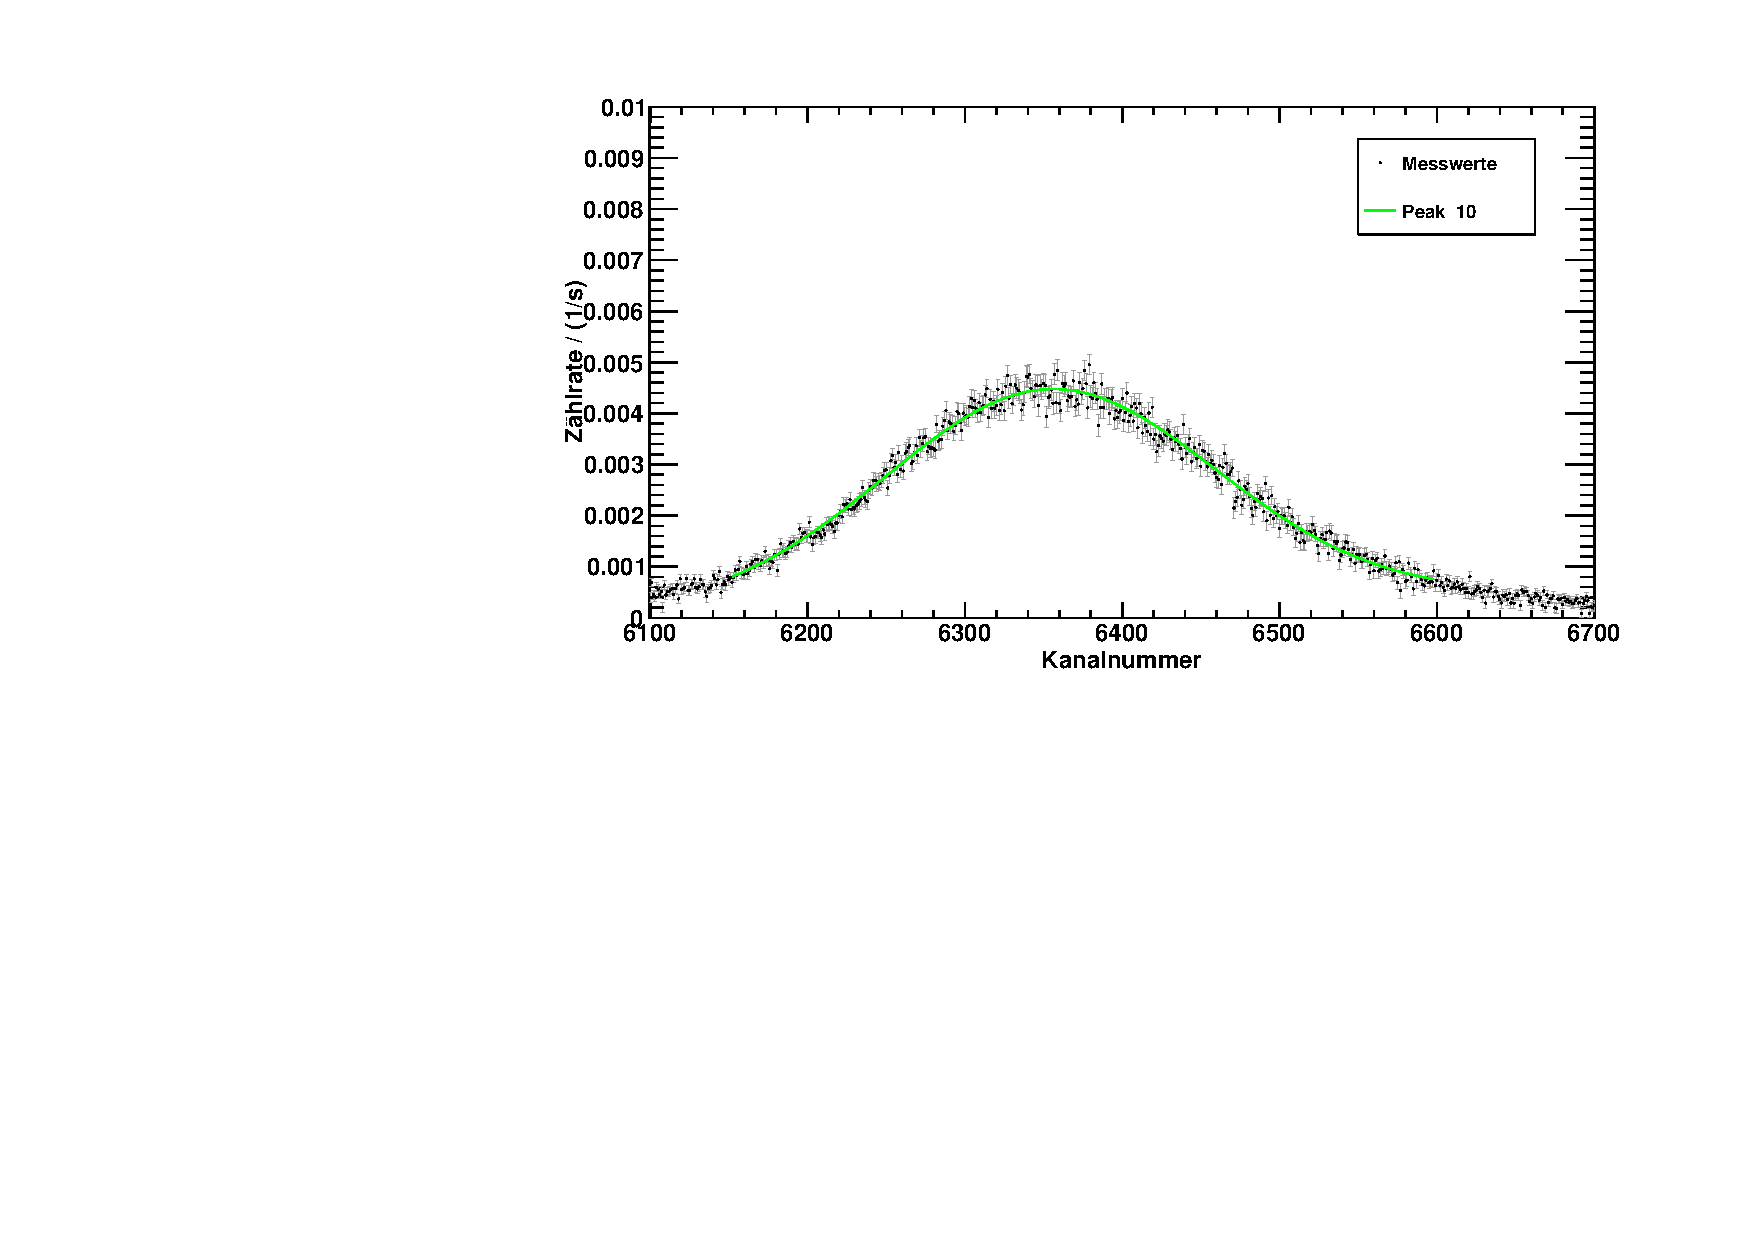
\includegraphics[width=\textwidth]{../img/th_peaks_single_10.pdf}
  \caption{Peak 10}
  \label{img:th:peaks:single:10}
\end{center}
\end{figure}

\subsubsection{Multi-Peak Fit} % TODO Benennung
\begin{figure}[H]
\begin{center}
  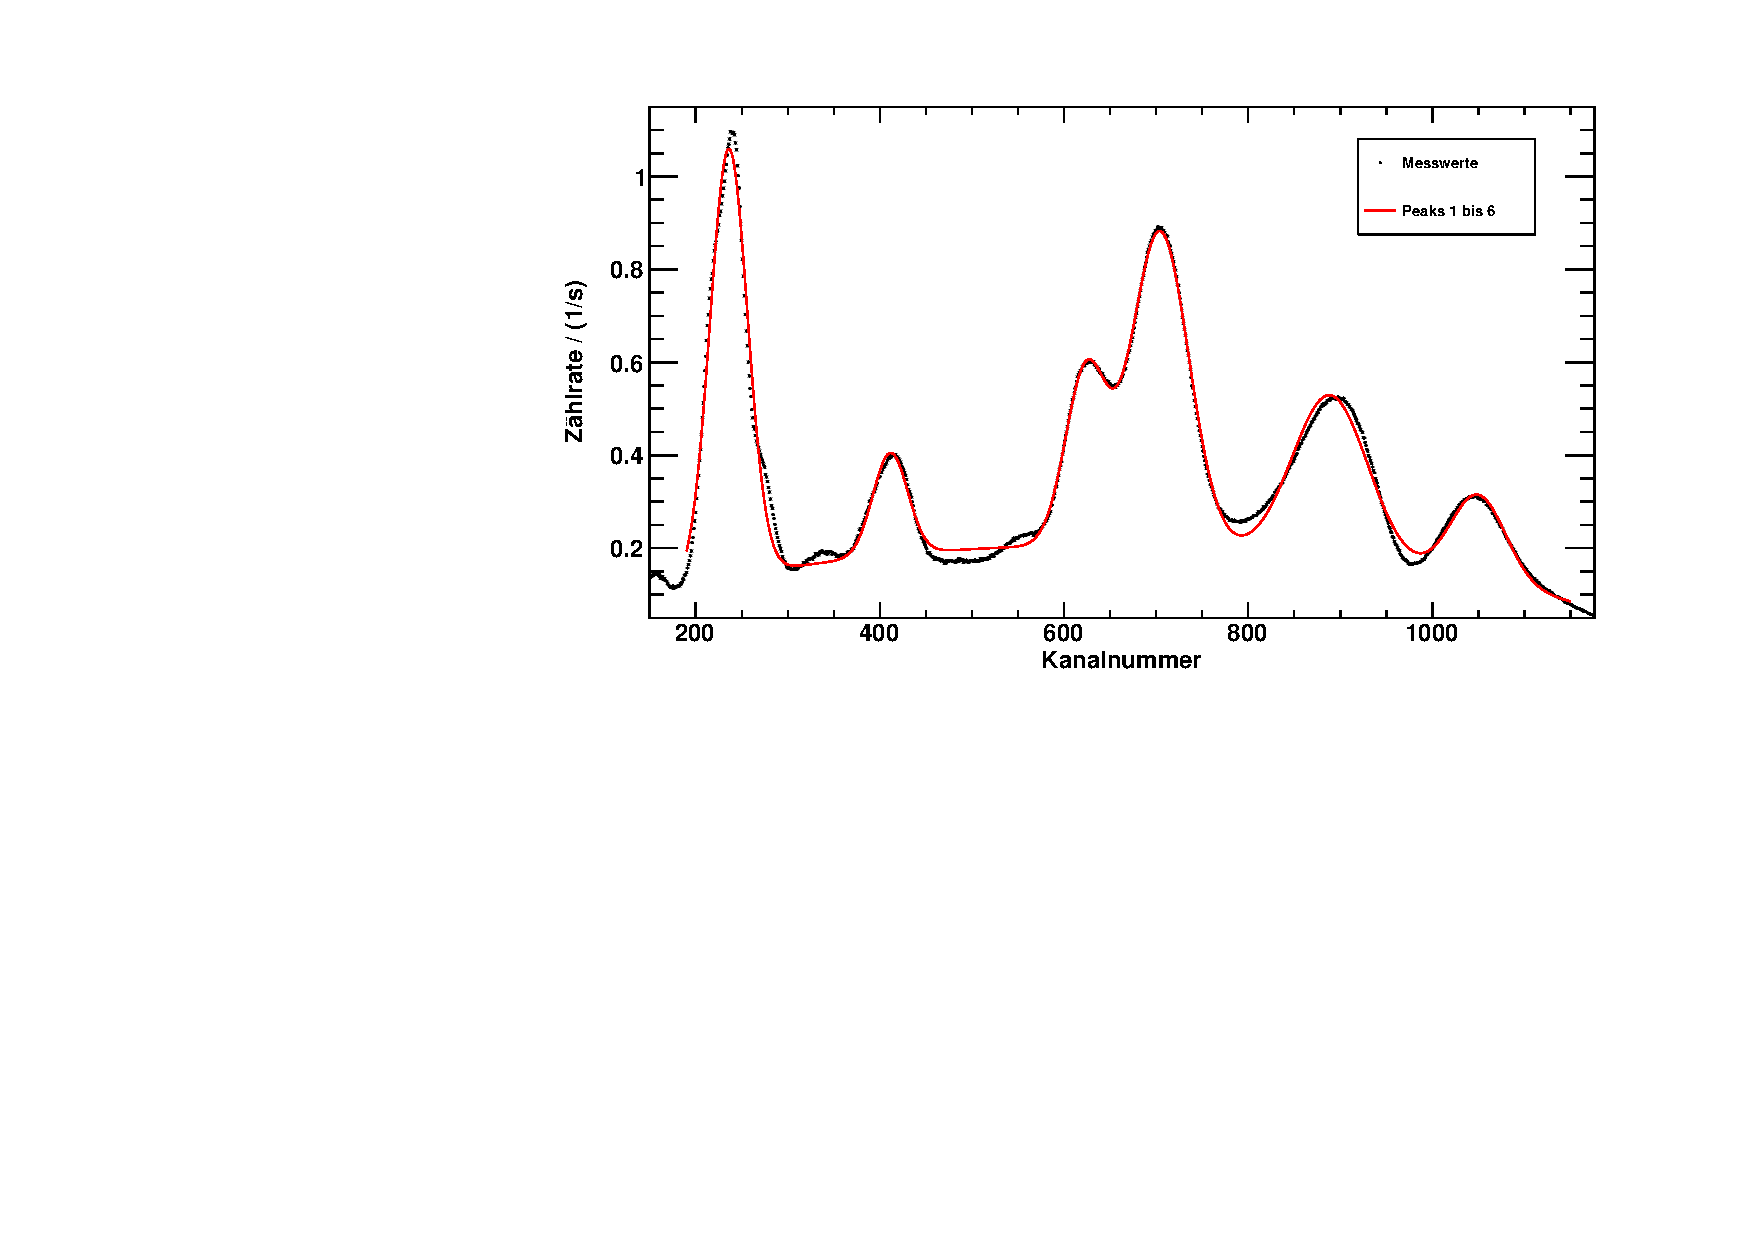
\includegraphics[width=\textwidth]{../img/th_peaks_multi_01-06.pdf}
  \caption{Peaks 1 bis 6}
  \label{img:th:peaks:multi:0106}
\end{center}
\end{figure}

\begin{figure}[H]
\begin{center}
  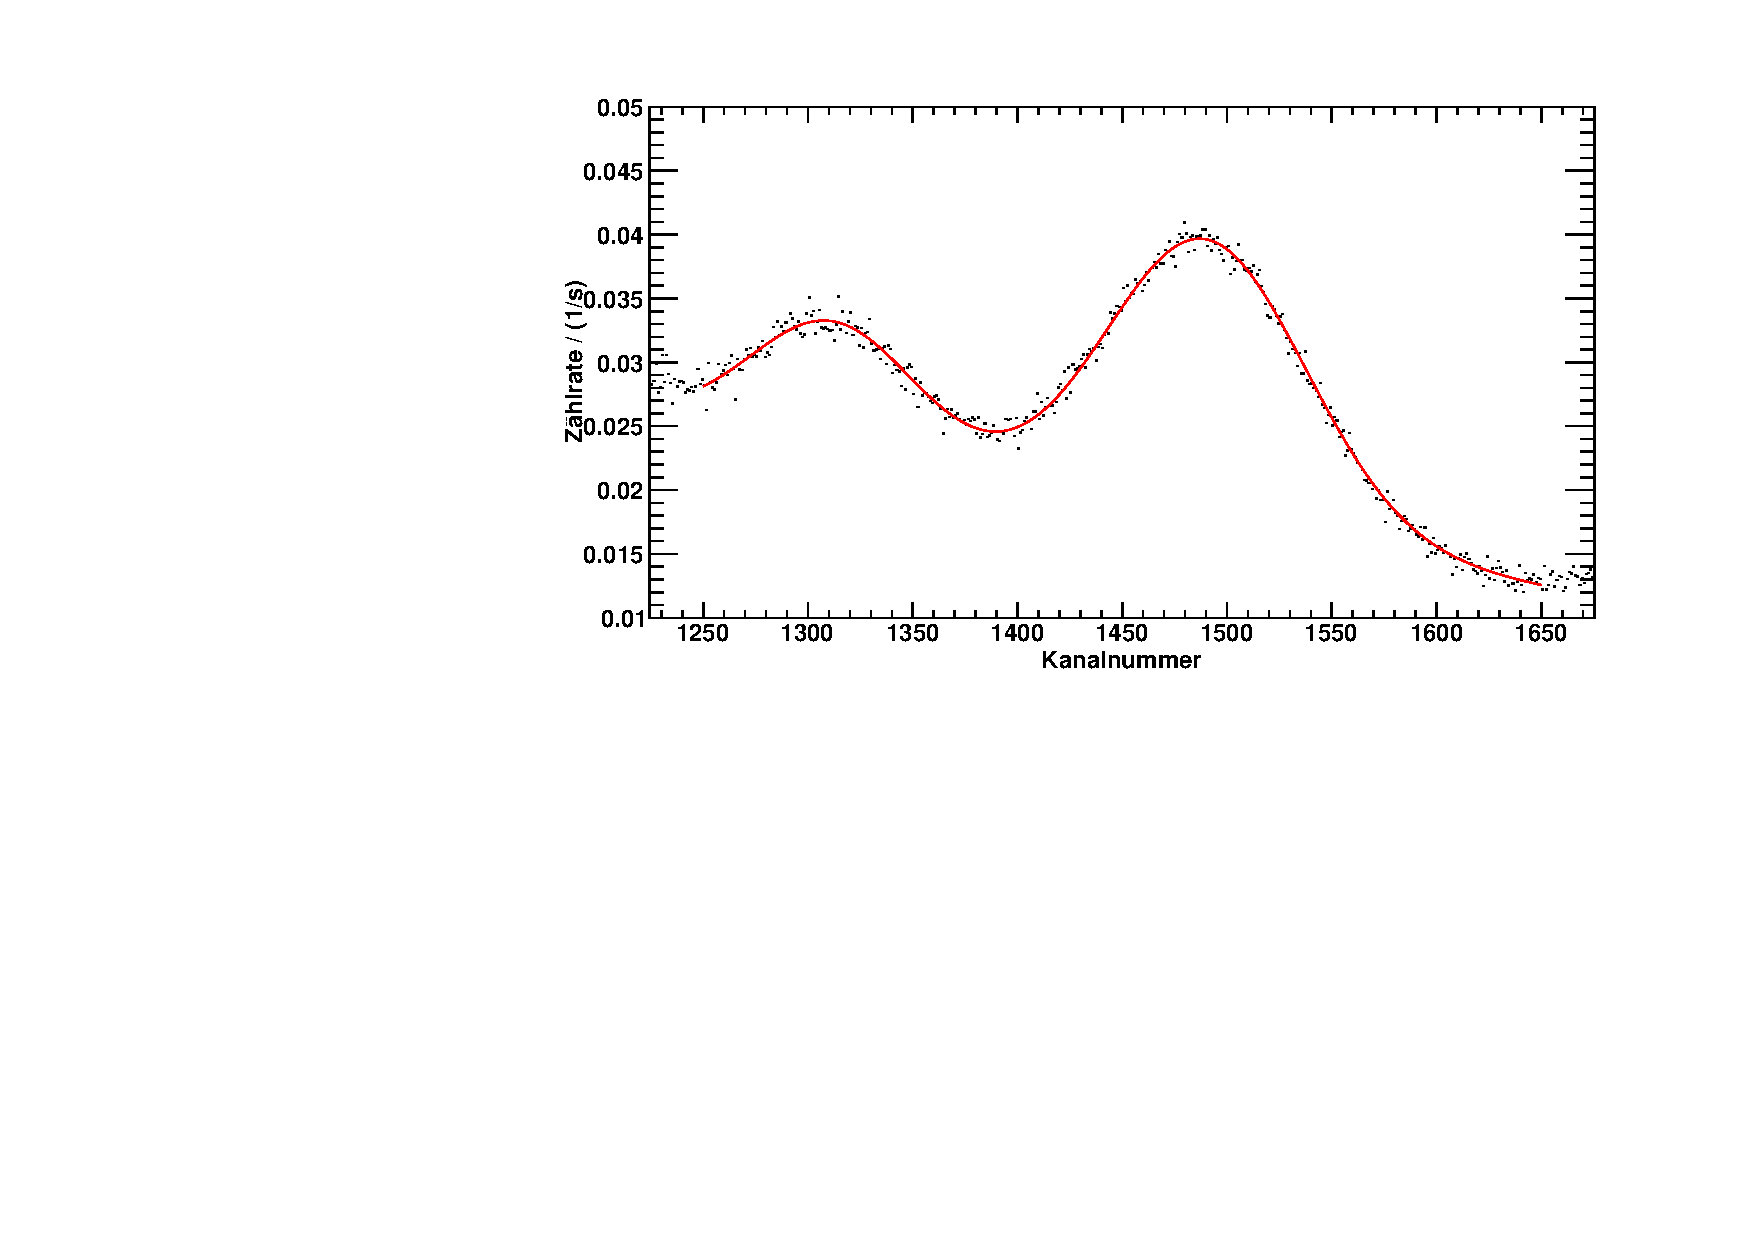
\includegraphics[width=\textwidth]{../img/th_peaks_multi_07-08.pdf}
  \caption{Peaks 7 und 8}
  \label{img:th:peaks:multi:0708}
\end{center}
\end{figure}

\subsection{Untergrundpeak}
\label{sub:eval:undergroundpeak}

\subsection{Winkelkorrelation der \chemel{Na}{22} Vernichtungsphotonen}
\begin{figure}[H]
\begin{center}
  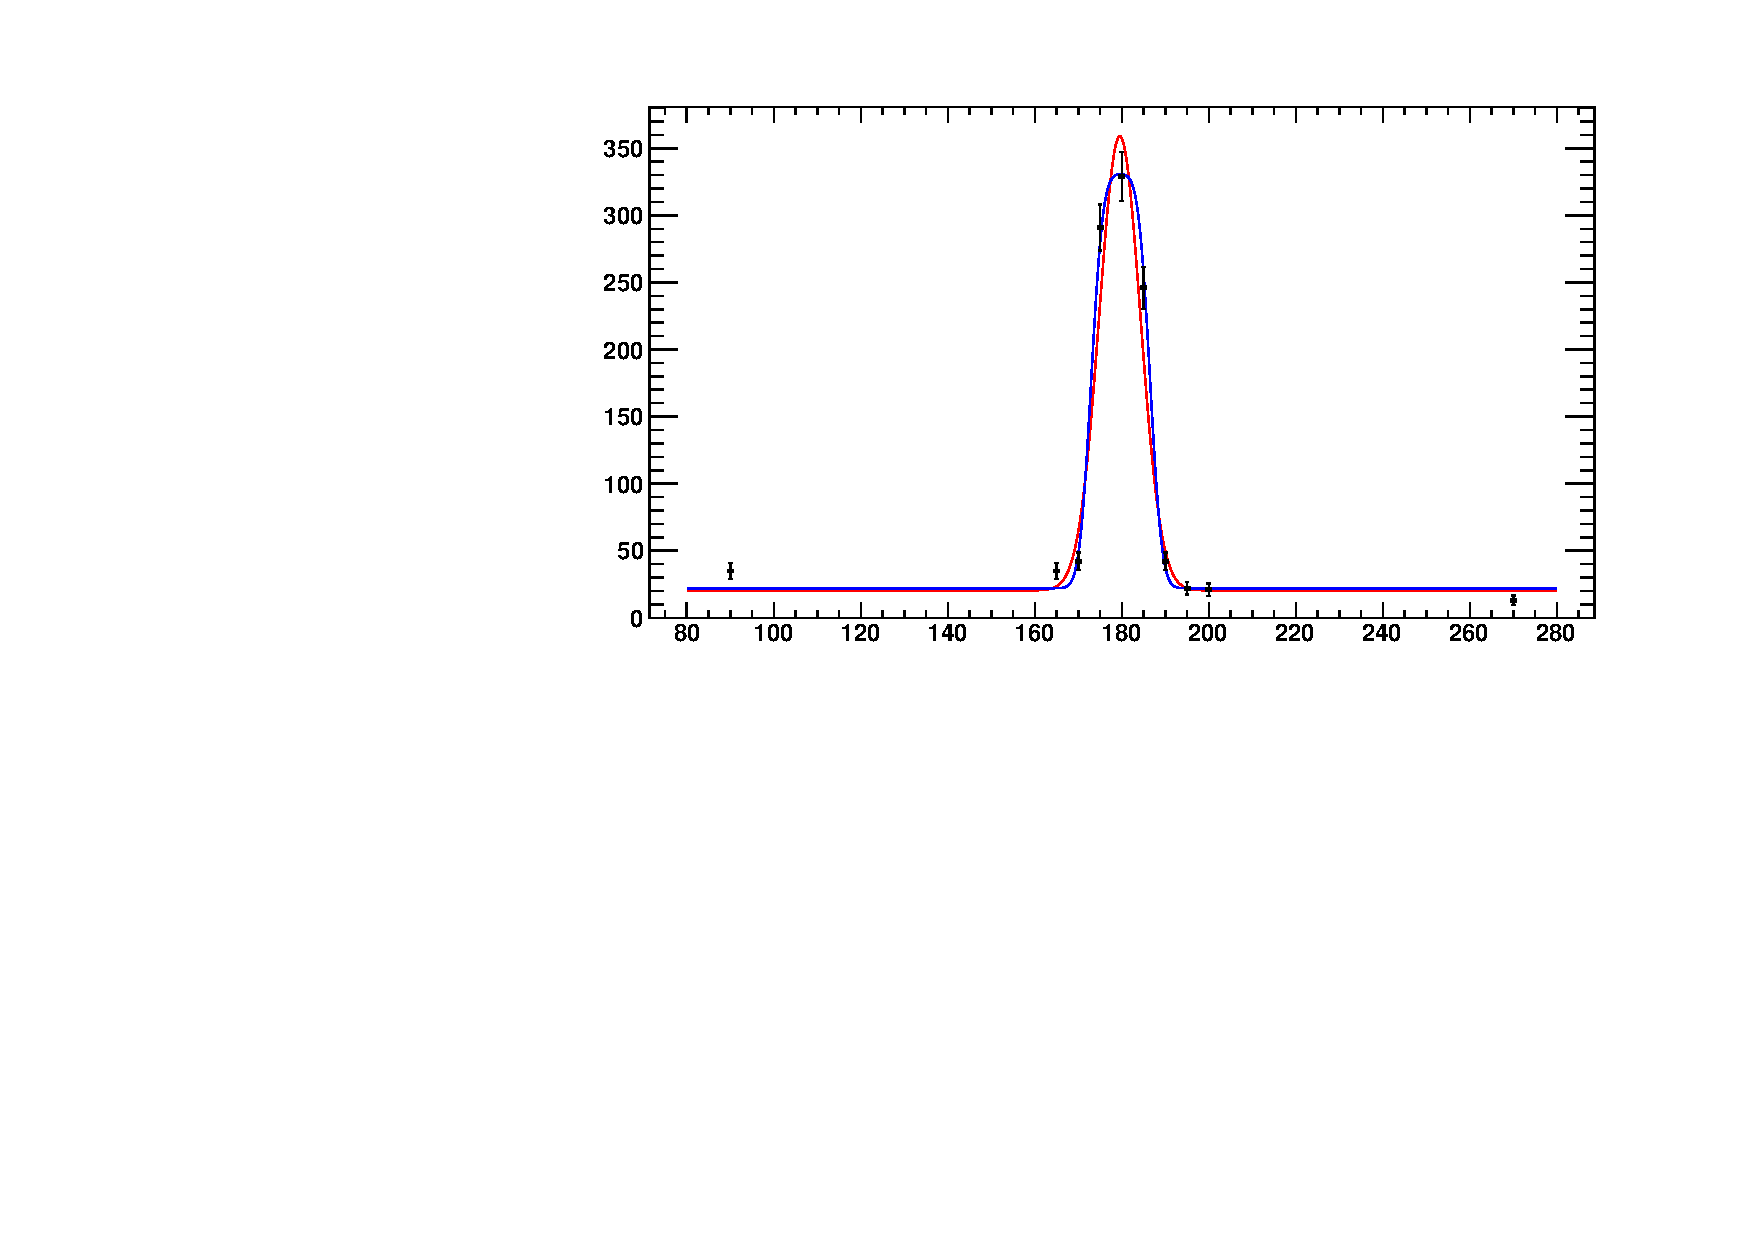
\includegraphics[width=\textwidth]{../img/angles.pdf}
  \caption{Winkelkorrelation der \chemel{Na}{22} Vernichtungsphotonen}
  \label{img:angles}
\end{center}
\end{figure}
